\typeout{NT FILE DESIGN.tex}%
\chapter{Design}%
\label{ch:design}
%
This chapter presents the design of a trustworthy flight software stack tailored
for a typical UAV application --- video surveillance --- leveraging the Bao
hypervisor. Firstly, the system requirements and constraints are systematically
identified. Then, we analyze the conventional solution consisting of a
\gls{umpfs}: the flight controller hardware node manages flight-critical
systems, while the companion computer hardware node handles secondary and
computationally intensive tasks, such as collision avoidance and prevention,
odometry, or, in this case, video streaming to the \gls{gcs}. This solution
handles mixed-criticality at the hardware level, undesirably increasing the
footprint and weight of the \gls{uav}. Furthermore, it does not provide
isolation guarantees, thus compromising the companion computer can lead to the
flight controller's malfunctioning, and consequently, in the worst case scenario
to the crash of the \gls{uav}.

To minimize the weight and footprint of the \gls{uav} we propose the merge of
the flight controller and companion computer into a single platform. This
integration reduces the separation of concerns: the same platform is now
responsible for both critical and non-critical tasks. However, this
consolidation can adversely affect system performance, particularly for critical
tasks, potentially compromising flight safety. Additionally, system security may
be weakened, as an attacker only needs to exploit vulnerabilities in a single
platform to compromise the entire system.

On its own, the \gls{uspfs} may not represent an improvement over the
conventional approach. While it reduces the system footprint and communication
latency between components, these benefits may come at the cost of diminished
performance and heightened safety and security risks. However, it is
hypothesized that this solution serves as an intermediate step toward a unified
platform capable of managing both critical and non-critical tasks through
appropriate supervision. This hypothesis underpins the proposed solution,
referred to as the \gls{sspfs}, which employs the Bao hypervisor.

\section{Requirements and Constraints}
\label{sec:req-sec}
Video surveillance missions necessitate geolocation control to survey a
designated target area and image acquisition to gather pertinent information
about that region. Both objectives can be achieved through offline or online
command methods, or a combination of the two.

In the offline command approach, the target area and the specific information to
be captured are well-defined and can be comprehensively specified \emph{a
priori} to the \gls{uav}. For instance, in cartographic applications, the UAV
systematically scans the target area to collect topographic data. Consequently,
the UAV can operate in a fully autonomous mode, with data being directly stored
in its onboard storage systems.

Conversely, the online command approach is more suitable for dynamic and
unpredictable environments, where the target area and relevant information are
not fully predefined. For example, in rescue missions, the identification of
targets is critical, necessitating active supervision by the \gls{gcs}. In this
context, the \gls{gcs} must have the capability to remotely control the \gls{uav} and receive real-time feedback, such as telemetry data and live video streams.

This example underscores the critical importance of the online command method,
which involves more stringent operational requirements. As a result, the primary
focus of this work will be on the online command approach.

\subsection{Requirements}
\label{sec:req}

\textbf{Functional}
  \begin{itemize}
    \item The \gls{gcs} must be able to remotely command the \gls{uav} and
obtain its geolocation in (soft) real-time 
    \item The \gls{gcs} must be able to capture images in (soft) real-time
    \item The \gls{uav} must have onboard control mechanisms to ensure stable
flight in compliance with the previous requirements
    \item The \gls{uav} must have flight autonomy (battery powered) 
    \end{itemize}


\textbf{Technical}
  \begin{itemize}
    \item The software stack must be fault-tolerant: if the video surveillance
application is compromised, the control system must remain online 
    \item The additional security and fault-tolerant mechanisms must not
increase significantly the flight control stack latency.
\item Merge the flight controller and companion computer into a single platform
to minimize the footprint and reduce latency, while respecting its
mixed-criticality characteristics
    \end{itemize}

\subsection{Constraints}
\label{sec:constr}

\textbf{Functional}
\begin{itemize}
    \item Minimize the \gls{uav}'s weight to enhance flight autonomy.
    \item Video surveillance requires high bandwidth; however, the remote
communication link of the \gls{uav} has a limited bitrate. The frame size must
be adjusted to ensure sufficient image quality for the mission. 
\end{itemize}


\textbf{Technical}
  \begin{itemize}
    \item The flight software stack must be open-source (e.g., PX4)
    \item Wireless communications are required for UAV's remote control and
image acquisition
\item The Bao hypervisor is used to provide additional security and
fault-tolerance to the flight control stack
    \end{itemize}

\section{System Architecture}
\label{sec:design-sysArch}
Fig.~\ref{fig:uav-design-conv-sol-1} illustrates the conventional solution ---
\gls{umpfs} --- tailored for the video surveillance application, which employs a
separation of concerns. In this approach, the flight controller hardware node
manages flight-critical systems, while the companion computer hardware node
handles secondary and computationally intensive tasks, such as collision
avoidance and prevention, odometry, or, in this case, video streaming to the
\gls{gcs}.

\begin{figure}[!hbt]
  \centering
  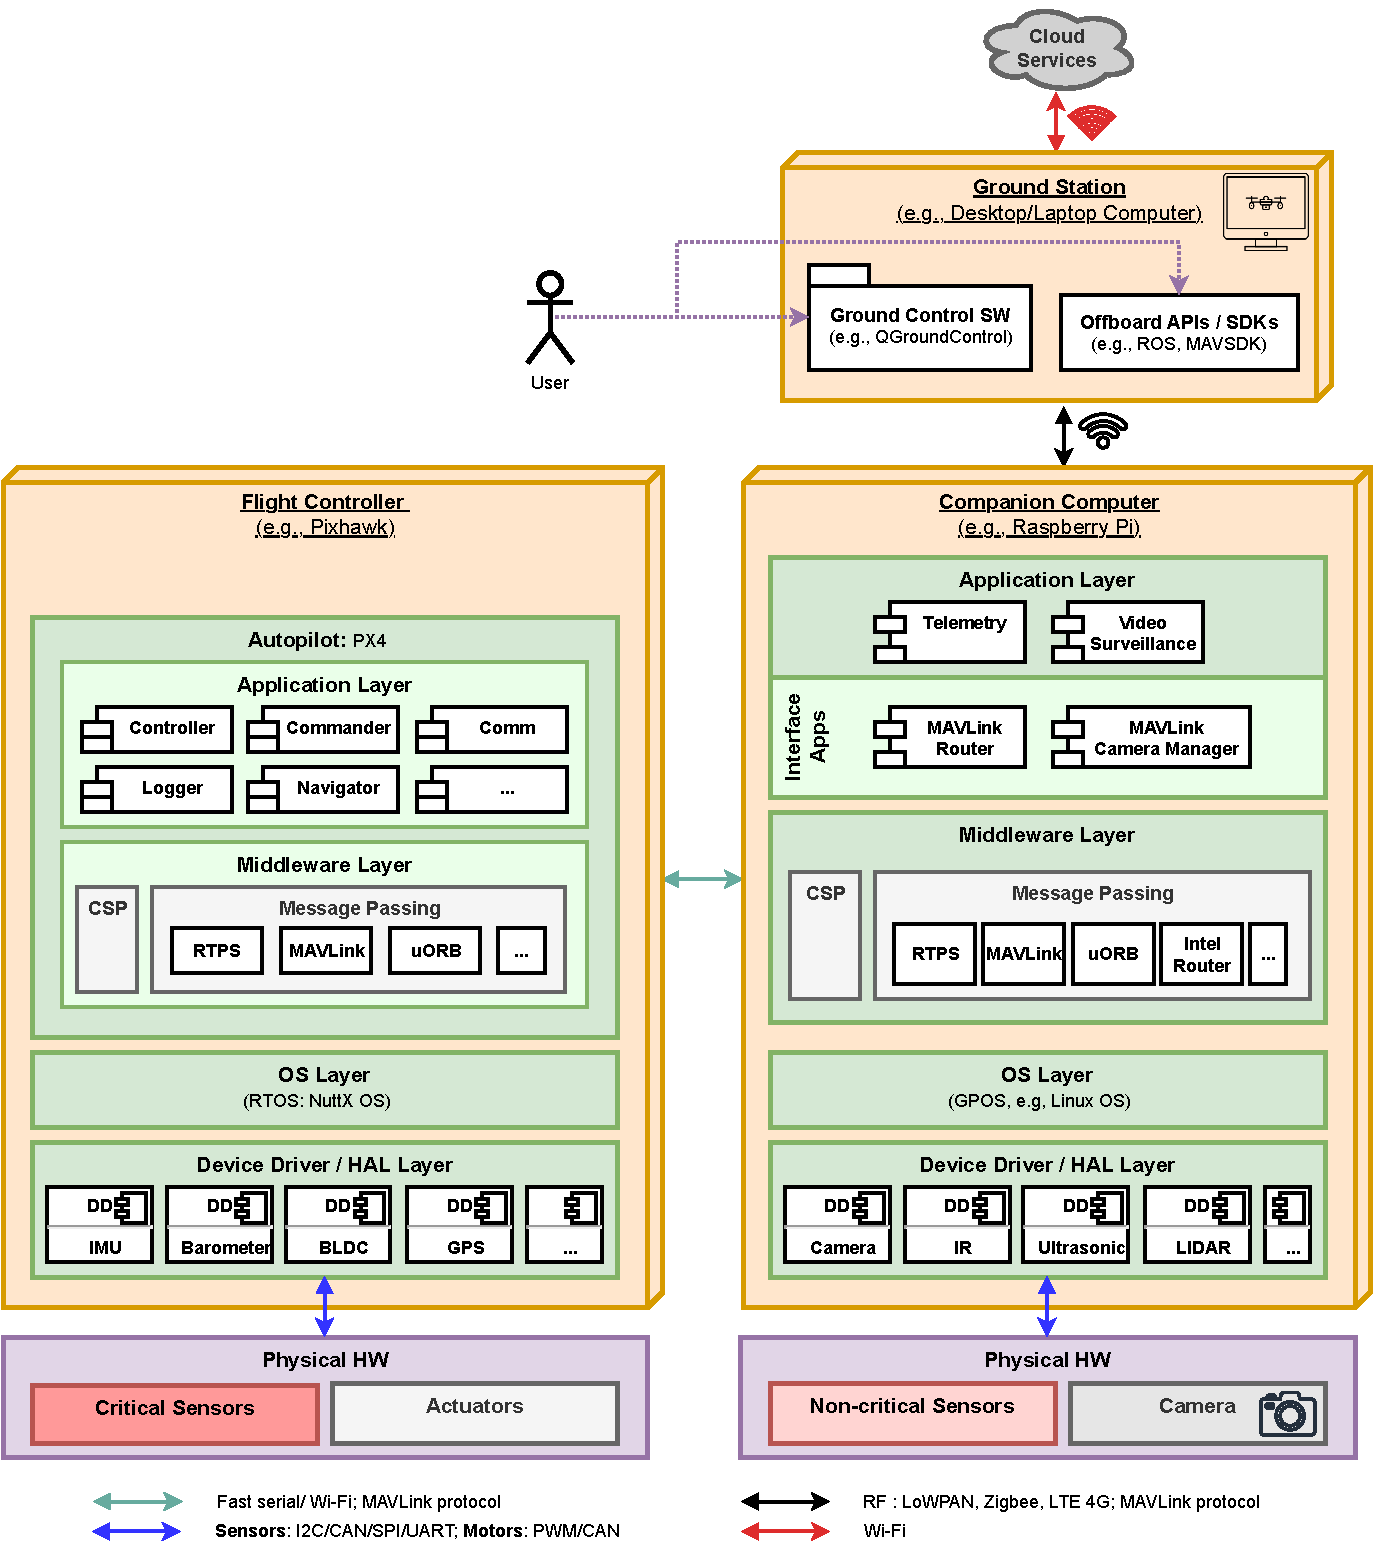
\includegraphics[width=1.0\textwidth]{./img/pdf/uav-main-design-conv-sol-1.pdf} 
%  \includesvg[width=1.0\textwidth]{./img/virtualization.svg} 
  %\caption[Virtualization mind map]{Virtualization mind map}%
  \caption{UAV design: conventional solution --- full}%
  \label{fig:uav-design-conv-sol-1}
\end{figure}

The PX4 flight controller stack was selected for this work due to its
open-source nature, extensive platform support, modular architecture, and
widespread adoption in the industry. PX4 runs on the flight controller on top of
the NuttX \gls{rtos}. In the generic case, the companion computer is used to
route communications between the \gls{gcs} and the \gls{fmu}: a fast serial
link, typically \gls{uart} or Ethernet, is established between the \gls{fmu} and
the companion computer using the MAVLink protocol; the companion computer
runs extra software to route the MAVLink traffic,
e.g. \href{https://github.com/mavlink-router/mavlink-router}{MAVLink
  Router}~\cite{px4-routers}.

The \texttt{User} interacts with the Ground Control \gls{sw}, namely
\texttt{QGroundControl}. \texttt{QGroundControl} was selected due to its
open-source nature and compatibility with the PX4 flight stack. Additionally,
the User can interact with the Companion Computer via offboard
\glspl{api}/\glspl{sdk}, e.g., \texttt{MAVSDK}. The \gls{rc} link was dropped,
as it is only usable in manual mode, thus, it is not useful for the video
surveillance application.

In the vast majority of cases, we also need extra software running on the companion
computer to interface the camera, e.g. the \href{https://github.com/mavlink/mavlink-camera-manager}{Mavlink Camera Manager}. This
component acts as bridge between the \gls{fmu} and \gls{gcs} and a translator between the MAVLink Camera Protocol v2
(used by PX4) and the native protocol of the camera~\cite{px4-cam-managers}.

The communications routing poses an increased risk to the \gls{uav}: if the
companion computer is compromised the \gls{fmu} may malfunction due to data
corruption or communication loss. Furthermore, the additional software required
to route MAVLink traffic and manage the camera adds complexity and latency to
the system.

Fig.~\ref{fig:uav-design-conv-sol-2} showcases a simplified conventional
solution customized for video surveillance, with a higher degree of
decoupling. Dedicated
communication links are established for communication between the \gls{gcs} and \gls{fmu} (telemetry radio) and the
camera (Wi-Fi). To streamline the network configuration and eliminate the need
for additional hardware, the \gls{gcs} and the \gls{uav} are integrated into the
same \gls{lan}. The video surveillance software is also simplified consisting of
a client running on the \gls{gcs} and the server running on the companion
computer supported by a suitable video pipeline and device drivers. The
client runs on port 5000 of the \gls{gcs} issuing command for the server running
on the same port in the Companion Computer. The server handles commands and
requests the sender to setup the video pipeline and transmit video frames back
to the \gls{gcs}. The receiver sets up a video pipeline on the \gls{gcs} (not
displayed) that processes the video frames and displays it to the \texttt{User}.

\begin{figure}[!hbt]
  \centering
  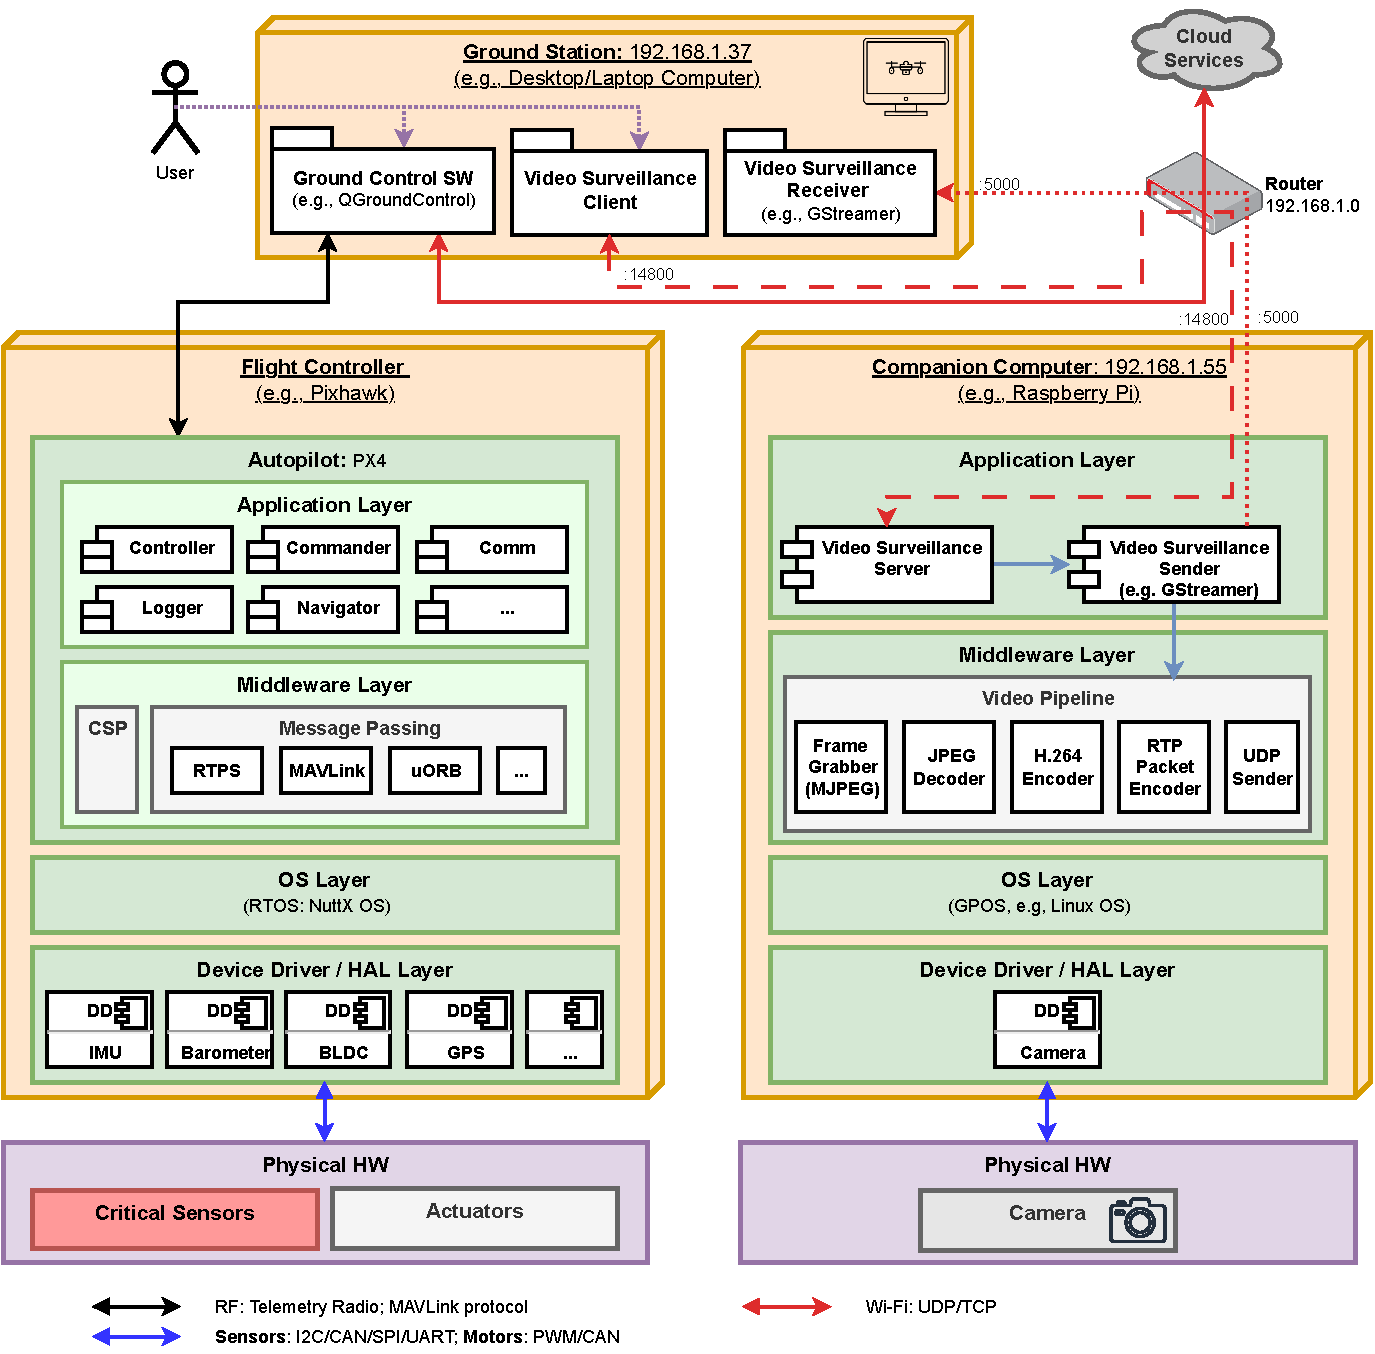
\includegraphics[width=1.0\textwidth]{./img/pdf/uav-main-design-conv-sol-2.pdf} 
%  \includesvg[width=1.0\textwidth]{./img/virtualization.svg} 
  %\caption[Virtualization mind map]{Virtualization mind map}%
  \caption{UAV design: conventional solution --- simplified}%
  \label{fig:uav-design-conv-sol-2}
\end{figure}

On the receiving end of the video surveillance system (\gls{gcs}), occasional frame loss is tolerable and does not compromise situational awareness of the target area. Consequently, a communication protocol without delivery guarantees, such as \gls{udp}, is appropriate.

This simplified conventional solution forms the base design for the platform
unification.

\subsection{Unsupervised Single-Platform Flight Stack}
\label{sec:unsuperv-stack}
To integrate the \gls{fmu} and companion computer platforms, we require a method to encapsulate their functionalities into standalone components within a unified platform. In the \acrfull{uspfs}, these components are abstracted as processes running on a \gls{gpos}.

Fig.~\ref{fig:uav-design-unsup} illustrates the system architecture of the
\gls{uspfs}. The software processes for the \gls{gcs} and \gls{uavic} are shown
in blue. The \gls{uavic} consolidates the \gls{fmu} and companion computer nodes
into a single platform operating on a \gls{gpos}, specifically Linux. PX4
executes on core 0, while the remaining cores are allocated for the video
surveillance application.

\begin{figure}[!hbt]
  \centering
  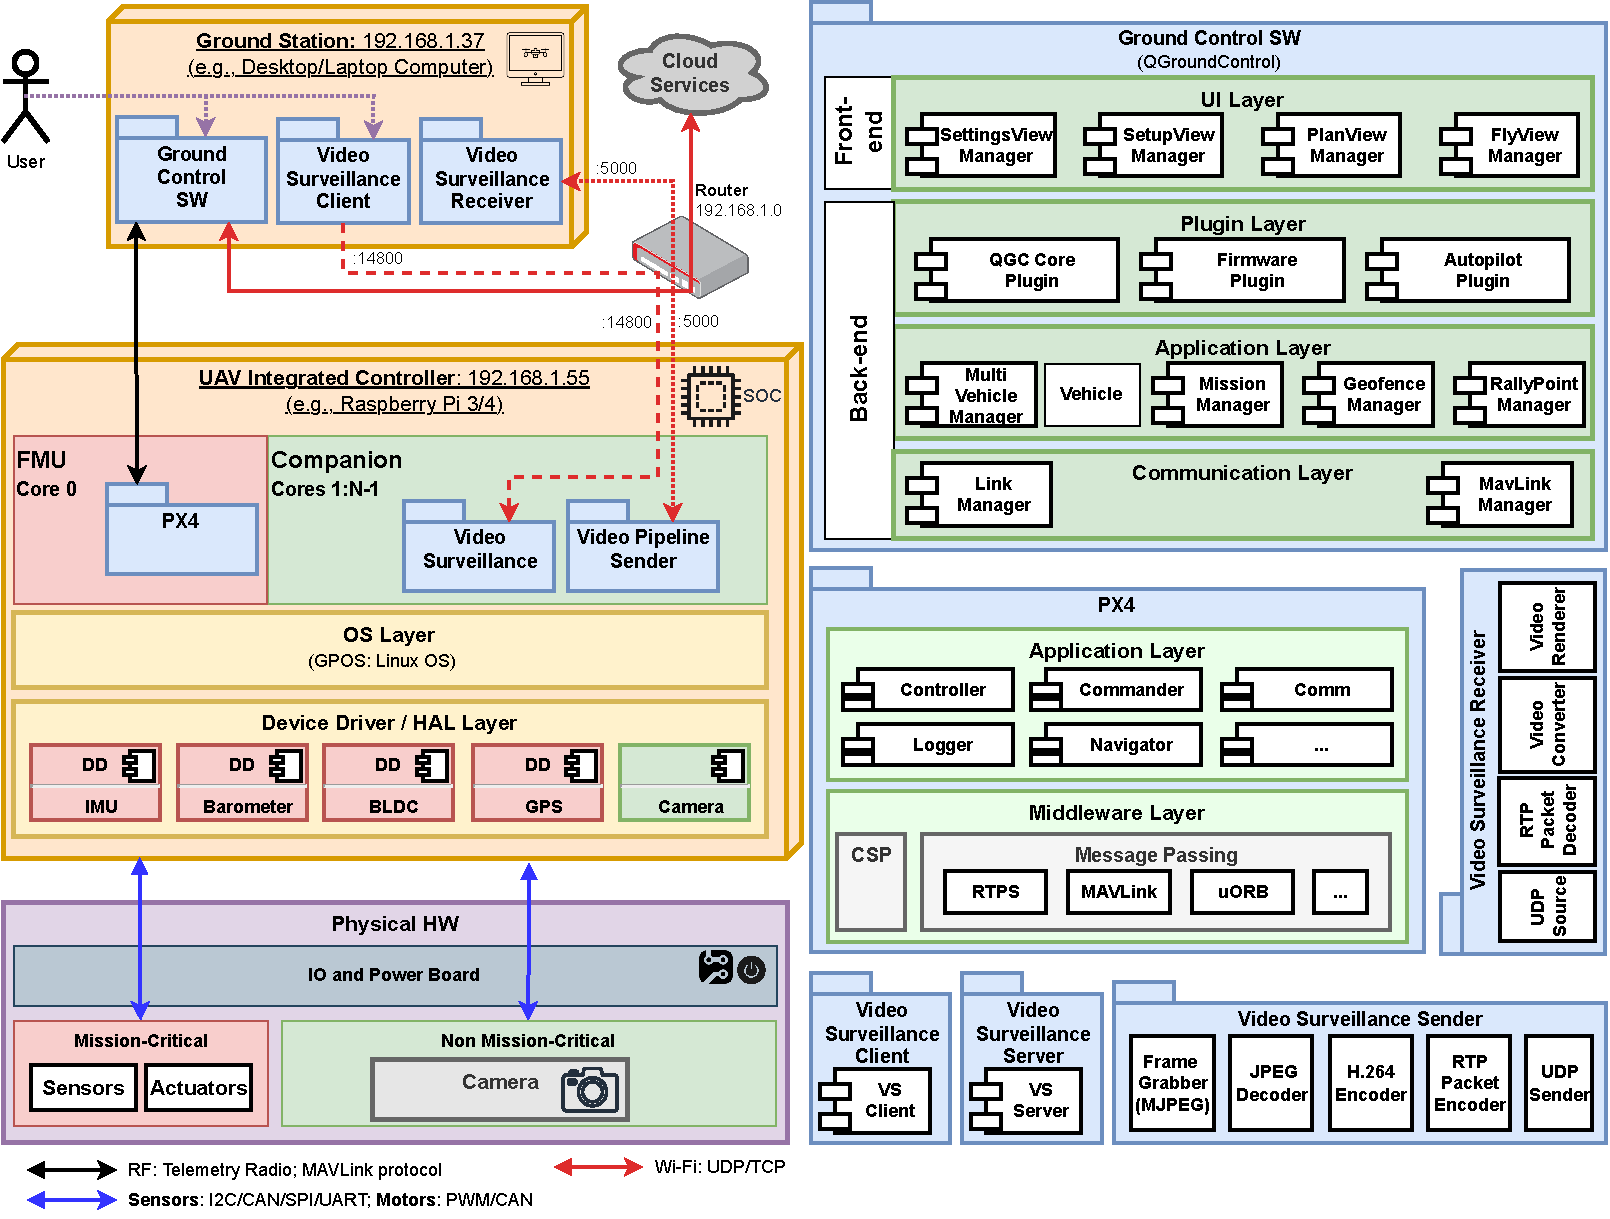
\includegraphics[width=1.0\textwidth]{./img/pdf/uav-main-design-unsup.pdf} 
%  \includesvg[width=1.0\textwidth]{./img/virtualization.svg} 
  %\caption[Virtualization mind map]{Virtualization mind map}%
  \caption{UAV design: Unsupervised Single-Platform Flight Stack}%
  \label{fig:uav-design-unsup}
\end{figure}

It is important to note that PX4 no longer runs on the Nuttx \gls{rtos}, which may introduce challenges in meeting the soft real-time requirements of flight control. To address this, one core is explicitly dedicated to the PX4 application. Additionally, employing a real-time Linux kernel with a suitable \gls{io} scheduler can help mitigate timing issues.

However, this architecture lacks isolation between systems, meaning a failure in the non-critical system can propagate to the \gls{fmu}. Such failures could lead to \gls{fmu} malfunctions, potentially resulting in a crash with unpredictable consequences. As mentioned earlier, this solution alone is insufficient; supervision is essential to ensure both reliable consolidation and safe integration.

\subsection{Supervised Single-Platform Flight Stack}
\label{sec:superv-stack}
Fig.~\ref{fig:uav-design-unsup} presents the system architecture of the
\acrfull{sspfs}. In this design, the functionalities of the \gls{fmu} and
companion computer are abstracted as guest \glspl{vm} running atop the Bao
Hypervisor in the \gls{uavic} node. This approach ensures isolation between the two mixed-criticality
systems, preventing faults in the non-critical system from impacting the
\gls{fmu} and causing potential malfunctions.

\begin{figure}[!hbt]
  \centering
  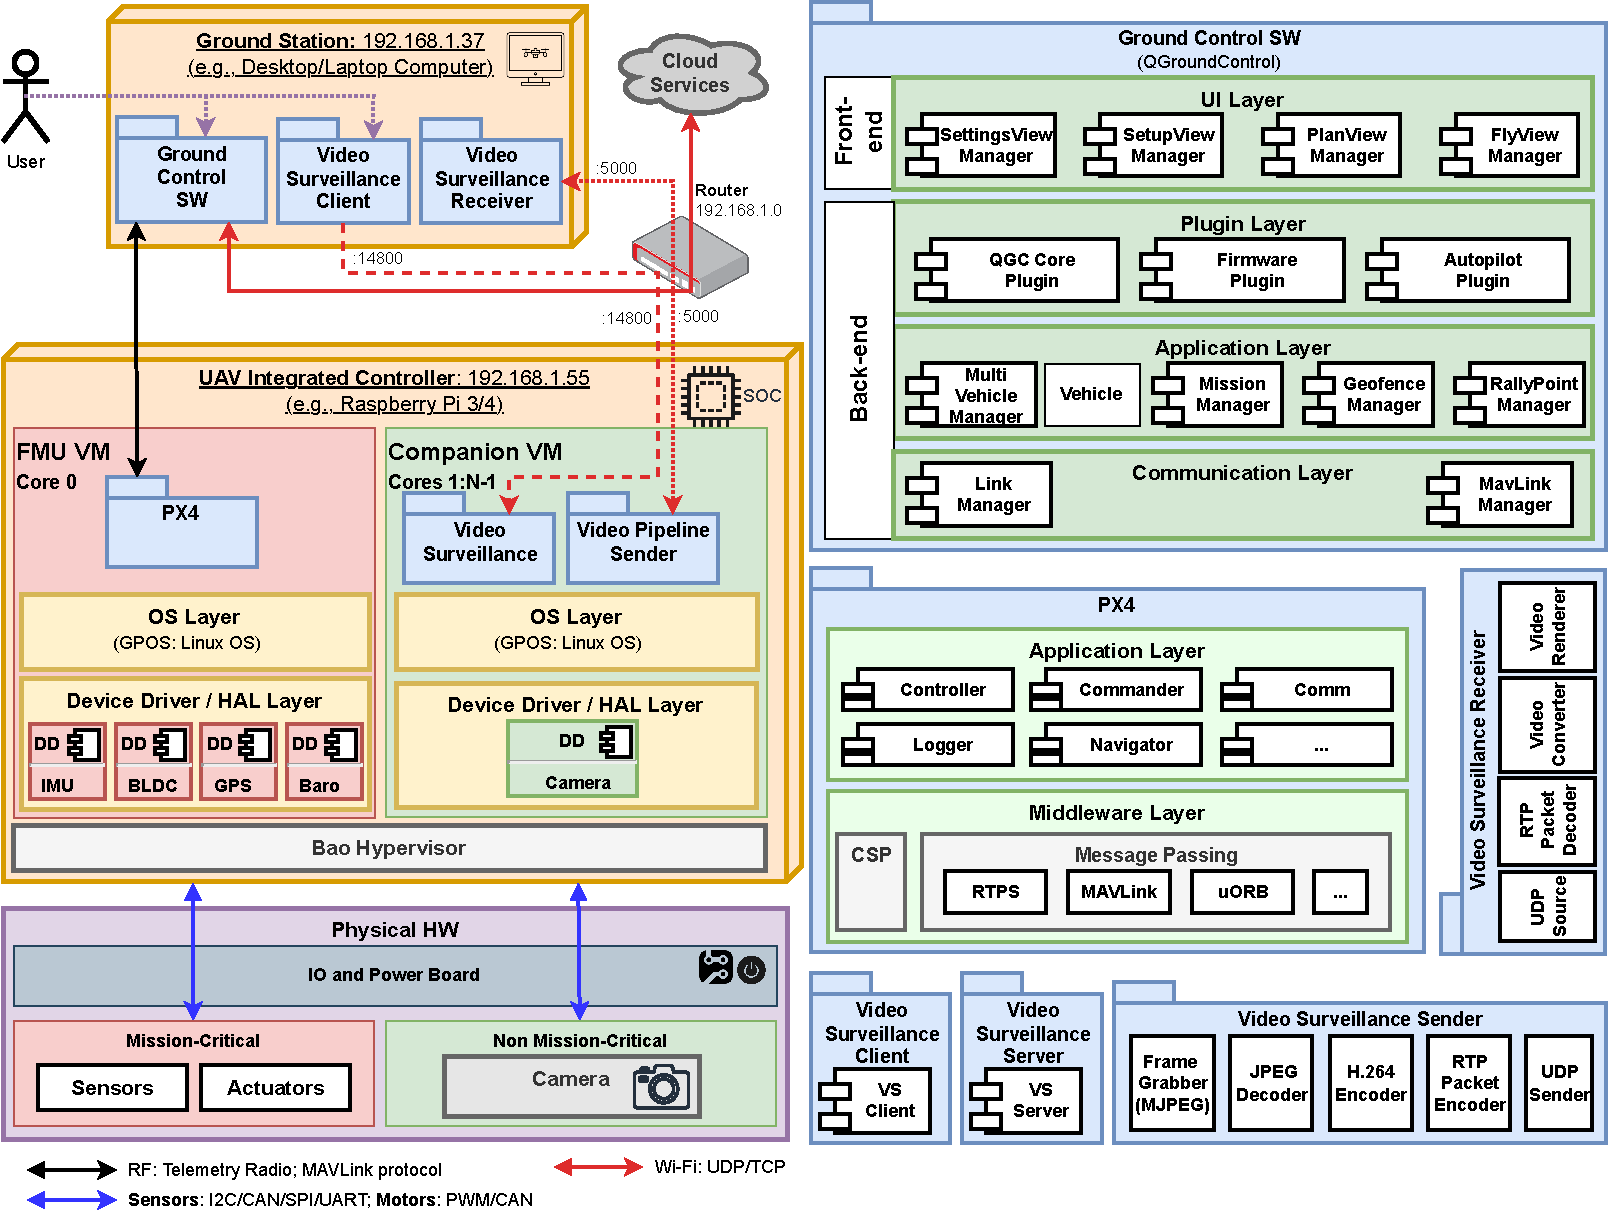
\includegraphics[width=1.0\textwidth]{./img/pdf/uav-main-design-sup.pdf} 
%  \includesvg[width=1.0\textwidth]{./img/virtualization.svg} 
  %\caption[Virtualization mind map]{Virtualization mind map}%
  \caption{UAV design: Supervised Single-Platform Flight Stack}%
  \label{fig:uav-design-sup}
\end{figure}

Each \gls{vm} operates a Linux-based \gls{os}, enabling further customization. For instance, the \gls{fmu} \gls{vm} can utilize a real-time kernel, providing additional guarantees that its assigned core remains fully dedicated to its execution. Meanwhile, the Companion \gls{vm} can operate with a standard Linux kernel. Bao's static partitioning mechanism guarantees that the hardware resources assigned to each \gls{vm} are strictly dedicated, ensuring isolation. Moreover, device drivers within each \gls{vm} are specific to that \gls{vm}, minimizing the impact of software bugs or failures.

However, this approach requires each \gls{vm} to include a full \gls{os},
leading to larger binary sizes. Additionally, the \texttt{User} must carefully
select and allocate hardware resources to avoid conflicts between \glspl{vm}
while maintaining adequate performance in terms of \gls{ram}, available
\glspl{cpu}, and other critical resources. This requires a deeper knowledge
about the hardware used. As such, we will later revisit the system architecture
to adapt it to the selected hardware.

\section{Hardware Selection}
\label{sec:hardware-selection}




%%% Local Variables:
%%% mode: latex
%%% TeX-master: "../template"
%%% reftex-default-bibliography: ("../Bibliography/mieeic.bib")
%%% ispell-local-dictionary: "american"
%%% End:
